\chapter{Przegląd dostępnych rozwiązań}
\label{cha:przegladRozwiazan}

{\it

	Istnieje szereg dostępnych rozwiązań implementujących mechanizmy gwarantowania bezpieczeństwa dostępu do aplikacji. Z perspektywy pracy najbardziej interesującymi przykładami rozwiązań tego typu są standardy realizujące założenia systemów zarządzania tożsamościami. Niniejszy rozdział przedstawia najbardziej popularne specyfikacje oparte o koncepcje zarządzania tożsamościami - SAML, OpenID oraz Liberty Identity Web Services Framework. Najbardziej istotnym z punktu widzenia pracy standardem jest oparta na języku XML specyfikacja SAML. SAML pozwala na wymianę informacji o tożsamości użytkowników pomiędzy komponentami systemu informatycznego oraz definiuje przebieg procesów komunikacji wykonywanych w celu potwierdzenia tożsamości klientów aplikacji. Określa również format wymienianych wiadomości. 

	W wielu systemach rozproszonych wykorzystywane są mechanizmy uwierzytelniania i autoryzacji oparte o koncepcje różne niż systemy zarządzania tożsamościami. Jednym z popularnie stosowanych standardów jest protokół Kerberos. System Kerberos realizuje mechanizmy jednokrotnego uwierzytelniania użytkowników aplikacji poprzez wprowadzenie koncepcji biletów ogólnego przeznaczenia, dzięki którym przyznawane są bilety dedykowane konkretnym usługom żądanym przez użytkownika.

	Opracowano również szereg standardów ukierunkowanych na zapewnienie bezpieczeństwa dostępu do usług webowych opartych o protokół SOAP. Wśród nich wymienić można - WS-Security(definiujący mechanizmy uwierzytelniania oraz sposoby gwarantowania poufności i integralności przesyłania komunikatów), WS-Trust(określający mechanizmy wymiany informacji o tożsamościach pomiędzy różnorodnymi usługami) oraz WS-Federation(umożliwiający współdzielenie tożsamości użytkowników pomiędzy różnymi domenami bezpieczeństwa). Innym powszechnie stosowanym standardem w kontekście zapewniania bezpieczeństwa dostępu do aplikacji jest specyfikacja OAuth - definiująca mechanizmy autoryzacji realizowane przy użyciu protokołu HTTP. 

}

%---------------------------------------------------------------------------

\autsection{Najpopularniejsze standardy IdM}{Krzysztof Wilaszek}
\label{sec:standardyIdM}

Implementacja systemów zarządzania tożsamościami jest obszarem, w którym standaryzacja procesów wykorzystywania danych osobowych przynosi istotne korzyści. Wprowadzenie standardowych rozwiązań upraszcza wdrożenie nowych aplikacji lub usług typu ,,Identity Provider''. Ujednolicenie sposobu korzystania z funkcjonalności systemów zarządzania tożsamościami umożliwia tworzenie aplikacji klienckich używających podobnych rozwiązań dla dostępu do różnych usług. Rozwijanych jest wiele standardów realizujących wymagania stawiane systemom zarządzania tożsamościami. Najbardziej istotne z nich to SAML(Security Assertion Markup Language) oraz OpenID. 

\subsection{Security Assertion Markup Language}

	SAML to oparty na języku XML standard zarządzania tożsamościami oraz wymiany informacji uwierzytelniających \cite{Wisniewski05}. SAML oparty jest na podejściu wykorzystującym federację tożsamości - umożliwia tworzenie powiązań pomiędzy różnymi cyfrowymi tożsamościami użytkownika. SAML pozwala tworzyć asercje opisujące atrybuty tożsamości jednostki oraz przekazywać je do usług wymagających informacji identyfikujących swoich klientów.

	\subsubsection{Cele technologii SAML}

		Cele stawiane technologii SAML to\cite{Wisniewski05}:

		\begin{itemize}
		  \item niezależność od platformy - mechanizmy bezpieczeństwa powinny być niezależne od środowiska i implementacji usługi.
		  \item luźne powiązanie pomiędzy elementami wchodzącymi w skład infrastruktury opartej o wymianę komunikatów SAML
		  \item uproszczenie procesu uwierzytelniania z perspektywy klienta, np. poprzez wprowadzenie procedury SSO
		  \item redukcja kosztów administracyjnych poprzez zastąpienie wielu oddzielnych modułów bezpieczeństwa jednym wspólnym dla  różnych aplikacji
		\end{itemize}

	\subsubsection{Struktura specyfikacji SAML}

		Specyfikacja technologii SAML definiuje czterowarstwową strukturę, w skład której wchodzą asercje, protokoły, mapowania dla protokołów komunikacyjnych oraz profile. 
		Asercje zawierają informacje wymieniane pomiędzy aplikacjami, usługami ,,Identity Provider'' oraz użytkownikami. Protokoły, mapowania oraz profile definiują mechanizmy przetwarzania asercji.

		\paragraph{Asercje}\mbox{}\\
					
			Asercje są to wiadomości zawierające dane identyfikacyjne jednostek w systemie. Składają się z deklaracji tożsamości opisujących jednostki, wygenerowanych przez usługę ,,Identity Provider'' systemu SAML. Na podstawie otrzymanych deklaracji tożsamości jednostki dostawca usługi podejmuje decyzję o przyznaniu lub odmówieniu prawa dostępu do swoich zasobów. Również dostawcy usług mają możliwość tworzenia asercji w celu utworzenia zapytania do serwisu uwierzytelniającego o parametry transakcji określania tożsamości. 

			\subparagraph{Struktura asercji}\mbox{}\\
			
				\begin{figure}[h]
				\centering
					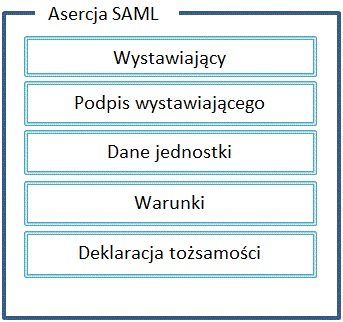
\includegraphics{img/samlAssertion.jpg}
				\caption{Elementy asercji SAML}
				\label{Elementy asercji SAML}
				\end{figure}

				Asercja SAML zawiera informacje o wystawiającym asercję. Może zawierać również informację o dacie wygenerowania asercji. W celu zapewnienia integralności informacji do asercji dołączany jest cyfrowy podpis wystawiającego. W dalszej części asercji znajdują się dane opisujące jednostkę, względem której utworzono asercję. Następną sekcją wiadomości są warunki, pod którymi asercja może być wykorzystywana. W tym fragmencie mogą znajdować się informacje o okresie ważności asercji lub usługi, do których adresowana jest asercja. Ostatnim elementem jest deklaracja tożsamości, zawierająca informacje kontekstowe o procesie uwierzytelniania, np. dotyczące zastosowanej metody uwierzytelniania.

			\subparagraph{Typy deklaracji tożsamości}\mbox{}\\

				Specyfikacja definuje następujące typy deklaracji tożsamości zawartych w asercjach SAML\cite{Wisniewski05}:

				\begin{itemize}
				  \item deklaracja uwierzytelniania - stwierdza, że opisana w asercji jednostka została uwierzytelniona w danym momencie przy użyciu mechanizmów opisanych w opisie kontekstu deklaracji
				  \item deklaracja atrybutu - stwierdza, że dany atrybut o zadanej wartości jest przypisany jednostce
				  \item deklaracja autoryzacji - stwierdza, że jednostce opisanej w asercji przyznano lub odmówiono praw dostępu do zasobów pod określonymi warunkami
				 \end{itemize}

		\paragraph{Protokoły}\mbox{}\\ 

			Protokoły SAML definiują format wiadomości żądań i odpowiedzi pozwalających na komunikację pomiędzy elementami systemu zarządzania tożsamościami przy pomocy technologii SAML. Specyfikacja SAML określa protokoły:

			\begin{itemize}
			  \item protokół odpytywania usługi ,,Identity Provider'' o asercje
			  \item protokół żądania uwierzytelniania jednostki
			  \item protokół rejestrowania identyfikatorów jednostek
			  \item protokół żądania wygaśnięcia identyfikatora jednostki
			  \item protokół żądania jednokrotnego wylogowania z wielu aplikacji
			  \item protokół żądania odzwierciedlenia pomiędzy różnymi identyfikatorami jednostki
			\end{itemize}

		\paragraph{Mapowania dla protokołów komunikacyjnych}\mbox{}\\

			Mapowania SAML do protokołów komunikacyjnych określają w jaki sposób wiadomości protokołów SAML powinny być przekazywane przy pomocy standardowych protokołów komunikacyjnych.  Mapowania mogą np. definiować sposób przesyłania wiadomości SAML przy pomocy protokołów HTTP lub SOAP.

		\paragraph{Profile}\mbox{}\\

			Profile SAML definiują zbiór funkcjonalności jakie można uzyskać przy użyciu elementów niższych warstw(asercji, protokołów i mapowań) oraz sposób w jaki te funkcjonalności mogą być osiągnięte. Przykładem mogą być profile jednokrotnego uwierzytelniania specyfikujące sposób komunikacji pomiędzy dostawcami usług i serwisami ,,Identity Provider'' w celu dostarczenia mechanizmów SSO lub profile zapytania o asercję dla jednostki.

	\subsubsection{Mechanizmy jednokrotnego uwierzytelniania przy użyciu SAML}

		\paragraph{Schemat funkcjonowania mechanizmów SSO w oparciu o technologię SAML}\mbox{}\\

			\begin{figure}[h]
				\centering
					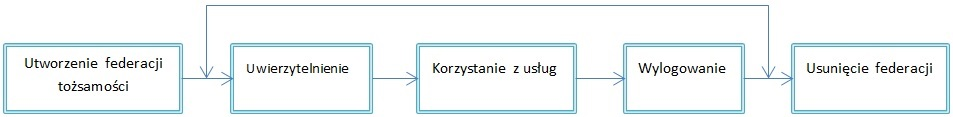
\includegraphics[width=15cm,height=2.5cm]{img/samlSSO.jpg}
				\caption{Schemat funkcjonowania mechanizmu jednokrotnego uwierzytelniania w SAML}
				\label{Schemat funkcjonowania mechanizmu jednokrotnego uwierzytelniania w SAML}
			\end{figure}

			Aby istniała możliwość korzystania z mechanizmu jednokrotnego uwierzytelniania konieczne jest utworzenie federacji pomiędzy tożsamościami jednostki. Po utworzeniu powiązań pomiędzy różnymi tożsamościami użytkownik po poprawnym uwierzytelnieniu względem jednej z usług może korzystać z innych sfederowanych serwisów. Wylogowanie się wykonane dla którejś z aplikacji powoduje zamknięcie dostępu do wszystkich sfederowanych usług. Procedura jednokrotnego uwierzytelniania może być wykorzystywana do momentu usunięcia federacji pomiędzy tożsamościami użytkownika.

		\paragraph{Przebieg procesu jednokrotnego uwierzytelniania w SAML}\mbox{}\\

			\begin{figure}[h]
				\centering
					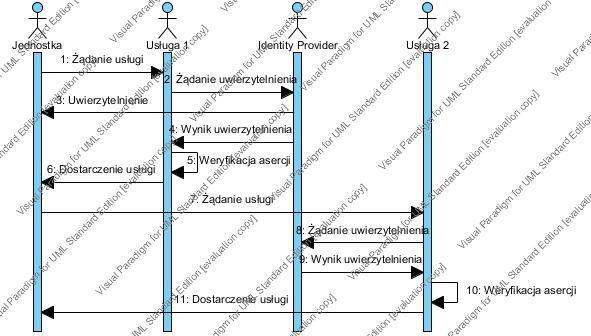
\includegraphics[width=15cm,height=10cm]{img/ssoSteps.jpg}
				\caption{Przebieg procesu jednokrotnego uwierzytelniania w SAML}
				\label{Przebieg procesu jednokrotnego uwierzytelniania w SAML}
			\end{figure}

			Usługa objęta mechanizmem jednokrotnego uwierzytelniania po otrzymaniu żądania udostępnienia swoich zasobów zleca modułowi ,,Identity Provider'' przeprowadzenie procesu uwierzytelnienia klienta serwisu. Asercja będąca wynikiem procesu uwierzytelnienia zostaje przekazana do usługi zlecającej. Usługa dokonuje weryfikacji otrzymanej asercji i akceptuje lub odrzuca żądanie dostępu do zasobów. Gdy użytkownik chce skorzystać z usług innego serwisu sfederowanego z usługą, do której otrzymał dostęp, proces uwierzytelniania przebiega podobnie. Pomijany jest jednak krok ponownego uwierzytelniania użytkownika przez usługę ,,Identity Provider'' - usługa ta zwraca do aplikacji żądającej uwierzytelniania asercję wygenerowaną na podstawie wcześniej wykonanego procesu uwierzytelniania.	
			
\subsection{OpenID}

	Standard \textit{OpenId} wykorzystuje podejście umożliwiające jednostkom dynamiczny wybór wykorzystywanej usługi typu \textit{,,Identity Provider''}. Specyfikacja oparta jest na koncepcji reprezentowania tożsamości jednostek przy użyciu identyfikatora URI(ang. \textit{Universal Resource Indicator}), dzięki czemu tożsamość może być wykorzystywana w dowolnej aplikacji korzystającej z sieci internet. Specyfikacja OpenID definiuje np. mechanizmy uwierzytelniania, wymiany atrybutów tożsamości jednostek oraz rejestracji jednostek. Istnieje wiele podobieństw pomiędzy standardami \textit{OpenId} oraz SAML jednak głównym wyróżnikiem specyfikacji \textit{OpenId} jest funkcjonalność wyszukiwania i dynamicznego wyboru usługi typu \textit{IdP}. Specyfikacja SAML określa jedynie format opisu lokalizacji usługi \textit{IdP}. \textit{OpenId} jest znacznie prostszy niż standard SAML - korzysta z mniej złożonych informacji o transakcjach bezpieczeństwa. Specyfikacja \textit{OpenId} nie definiuje funkcjonalności federacji tożsamości\cite{Bertino11}.

	\subsubsection{Uwierzytelnianie w standardzie OpenId}

		Standard \textit{OpenId} definiuje sposób dostarczania wyników uwierzytelniania jednostek do serwisów korzystających z usług \textit{IdP}. Klienci korzystający z usług wykorzystują asercje opisujące procesy uwierzytelniania przeprowadzone przez usługę \textit{,,Identity Provider''}. Protokół uwzględnia możliwość wykorzystania protokołu Diffiego-Hellmana w celu zestawienia bezpiecznego kanału komunikacyjnego pomiędzy dostawcą usług a serwisem \textit{IdP}. Wynikiem procesu uwierzytelniania jest asercja określająca jedynie czy proces zakończył się powodzeniem czy błędem. 

		\begin{figure}[h]
			\centering
			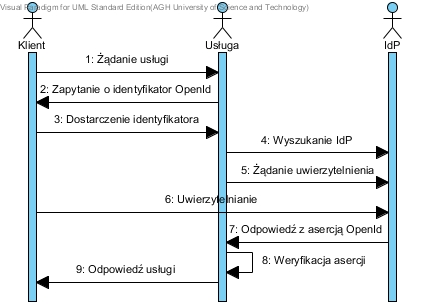
\includegraphics{img/OpenIdAuthentication.jpg}
			\caption{Przebieg procesu uwierzytelniania w standardzie OpenId}
			\label{OpenIdAuthentication}
		\end{figure}

		Klient przesyła żądanie dostarczenia usługi serwisu. Usługa wymaga uwierzytelnienia użytkownika - w tym celu przesyła żądanie dostarczenia identyfikatora \textit{OpenId} do klienta. Klient odpowiada przesyłając swój identyfikator. Serwis wyszukuje usługę \textit{IdP} na podstawie otrzymanego identyfikatora i przesyła do niej zapytanie o wynik procesu uwierzytelnienia. Usługa \textit{IdP} komunikuje się z klientem w celu przeprowadzenia procesu uwierzytelniania, generuje asercję zawierającą wynik oraz zwraca asercję do serwisu. Dostawca usług dokonuje weryfikacji otrzymanej asercji i na tej podstawie przyznaje klientowi dostęp do żądanych usług.

	\subsubsection{Pozostałe funkcjonalności definiowane standardem OpenId}

		Standard \textit{OpenId} definiuje rozszerzenia umożliwiające wymianę atrybutów zawartych w asercjach pomiędzy serwisem \textit{IdP} a dostawcą usług. Dostępne są dwie metody wymiany atrybutów - pobieranie wartości atrybutu z usługi \textit{Identity Provider} oraz ustawienie wartości atrybutu.

		Inne z rozszerzeń standardu \textit{OpenId} definiuje przebieg komunikacji pomiędzy serwisem \textit{Identity Provider} a dostawcą usług w celu dostarczenia informacji o politykach uwierzytelniania, które powinny być stosowane. Inne z rozszerzeń umożliwia dostawcom usług pobieranie atrybutów klienta od usługi \textit{IdP} za zgodą klienta.

\subsection{Liberty Identity Web Services Framework}

	Identity Web Services Framework(ID-WSF) to zbiór specyfikacji definiujących mechanizmy dla zapewnienia bezpieczeństwa serwisów webowych, pomiędzy którymi istnieją relacje zaufania(federacje)\cite{Oracle10}. ID-WSF określa podejście do zarządzania tożsamościami, w którym tożsamości jednostek zarządzane są przez różnych dostawców usług połączonych relacją federacji. Usługi webowe mogą wymieniać między sobą dane osobowe swoich użytkowników w celu dostarczenia funkcjonalności żądanej przez klienta usługi. Przykładem sytuacji, gdzie może być zastosowany ten model jest usługa potrzebująca dostarczenia danych adresowych swojego użytkownika. W tym celu może skorzystać z zasobów innej usługi dysponującej tymi danymi.

	Rysunek przedstawia przebieg procesu współdzielenia informacji w ID-WSF. Specyfikacja ID-WSF wprowadza dodatkowy element do architektury systemów zarządzania tożsamościami - ,,Discovery Service''. Usługa ,,Discovery Service'' pozwala dostawcom usług na wyszukiwanie innych serwisów dostarczających funkcjonalności pozwalających na realizację żądań zadanych usłudze. Klient aplikacji decyduje o tym czy jego dane mogą być dostępne dla innych serwisów rejestrując usługę dostarczającą jego danych osobowych w rejestrze ,,Discovery Service'' lub nie dokonując takiej rejestracji. Na przedstawionym schemacie żądana przez użytkownika usługa potrzebuje dodatkowych informacji - w tym celu w rejestrze usług szuka serwisu, który dostarcza potrzebnych informacji dla obsługiwanego użytkownika.

	\begin{figure}[h]
		\centering
			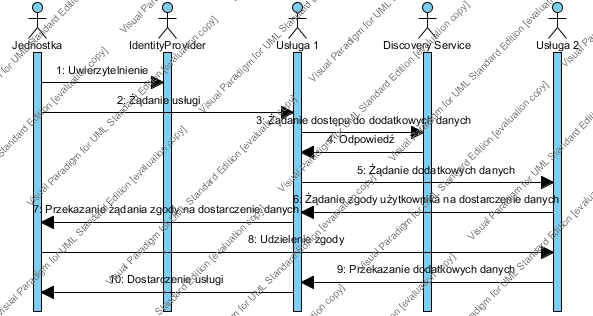
\includegraphics[width=15cm,height=9cm]{img/id-wsf.jpg}
		\caption{Przebieg procesu wykorzystywania informacji dzielonych w ID-WSF}
		\label{Przebieg procesu wykorzystywania informacji dzielonych w ID-WSF}
	\end{figure}

	ID-WSF definiuje również mechanizmy pozwalające na komunikację pomiędzy dostawcami usług i użytkownikiem w celu uzyskania zgody na przekazanie danych osobowych do innej aplikacji. Zaprezentowany diagram przedstawia ten proces. Usługa 2. po otrzymaniu żądania dostarczenia dodatkowych danych od Usługi 1. wymaga zgody użytkownika na udzielenie wymaganych informacji.
	
%---------------------------------------------------------------------------

\autsection{Przykłady frameworków zarządzających uwierzytelnianiem i autoryzacją użytkowników}{Krzysztof Wilaszek}
\label{sec:frameworki}

	\subsection{Protokół Kerberos}

		Kerberos jest protokołem uwierzytelniania użytkowników zasobów sieciowych.

		\subsubsection{Cele protokołu Kerberos}

			Centralnym punktem architektury Kerberos jest serwer uwierzytelniający\cite{Garman03}. Każdy komponent systemu Kerberos jest połączony z serwerem uwierzytelniającym relacją zaufania; wszystkie żądania uwierzytelniania są kierowane do tego serwera. Działanie systemu Kerberos opiera się na usługach KDC(Key Distribution Center). Każdy serwis KDC posiada bazę użytkowników i usług wraz z ich danymi uwierzytelniającymi. Dzięki temu możliwe jest uproszczenie zadań administracyjnych. Pozwala to również zastosować bardziej skuteczne mechanizmy bezpieczeństwa chroniące bazę użytkowników.

			Kerberos zapewnia bezpieczeństwo procesu uwierzytelniania gwarantując przesyłanie danych uwierzytelniających w postaci zaszyfrowanej. Korzysta z biletów(ang. Tickets) - wiadomości kryptograficznych dowodzących tożsamości użytkownika żądającego dostępu do zasobów serwera. Bilety dostarczane są przez usługę KDC na żądanie uwierzytelniającego się klienta. Bilety wystawiane są najczęściej na pewien okres - po jego upływie tracą ważność. Bazując na generowanych biletach Kerberos dostarcza mechanizm jednokrotnego uwierzytelniania. 

			Zastosowanie protokołu Kerberos gwarantuje obustronne uwierzytelnienie w procesie komunikacji pomiędzy klientem a serwerem - zarówno klient jak i serwer muszą dowieść swojej tożsamości. 

		\subsubsection{Elementy systemu Kerberos}

			Każdy użytkownik, usługa lub host w systemie Kerberos ma przypisany unikalny w ramach domeny identyfikator\cite{Garman03}. Każdy identyfikator skojarzony jest z kluczem uwierzytelniającym jednostkę w systemie. Kluczem tym może być np. hasło. Identyfikatory wraz z kluczami przechowywane są w bazie usługi ,,Key Distribution Center''. W skład KDC wchodzi również serwer uwierzytelniający i serwer TGS(Ticket Granting Server). W systemie Kerberos może istnieć więcej niż jedna usługa KDC - istnieje konieczność synchronizacji zawartości bazy identyfikatorów dla każdej z usług KDC.

		\subsubsection{Uwierzytelnianie w systemie Kerberos}

			\begin{figure}[h]
				\centering
					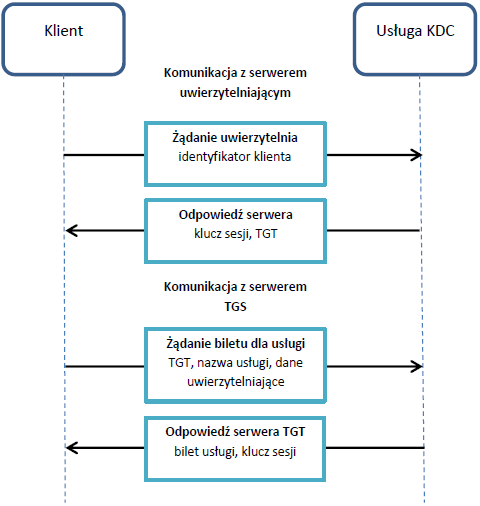
\includegraphics{img/kerberos.png}
				\caption{Przebieg procesu uwierzytelniania w protokole Kerberos}
				\label{Przebieg procesu uwierzytelniania w protokole Kerberos}
			\end{figure}

			Proces uwierzytelniania rozpoczyna się przesłaniem  do serwera uwierzytelniającego wiadomości żądania uwierzytelnienia wraz z opisem tożsamości klienta\cite{Garman03}. Serwer weryfikuje otrzymane informacje oraz znacznik czasowy dołączony do wiadomości - sprawdza w ten sposób czy żądanie nie zostało wygenerowano zbyt dawno. Po weryfikacji zakończonej sukcesem serwer generuje klucz sesji dzielony między klientem i serwerem TGS. Serwer przyznaje zaszyfrowany bilet - Ticket Granting Ticket(TGT) - użytkownikowi uwierzytelniającemu się w domenie. Serwer przesyła klucz sesji oraz tożsamość użytkownika zaszyfrowane kluczem serwera TGS oraz kopię klucza sesji szyfrowaną długoterminowym kluczem klienta. Dzięki temu użytkownik nie musi przesyłać usłudze swoich danych uwierzytelniających - dowodzi swojej tożsamości poprzez umiejętność odszyfrowania klucza sesji oraz biletu TGT. 

			Otrzymany bilet może być wykorzystany aby otrzymać bilet specyficzny dla zasobów, do których użytkownik chce uzyskać dostęp. Bilety specyficzne dla określonej usługi przyznawane są przez serwer TGS. Wiadomość przesyłana do serwera TGS składa się z żądania TGS, kopii biletu TGT oraz danych uwierzytelniających. Przesyłane dane uwierzytelniające obejmują znacznik czasowy szyfrowany kluczem sesji. Przesyłanie zaszyfrowanego znacznika czasowego pozwala zagwarantować, że klient ma dostęp do klucza sesji. Serwer dokonuje weryfikacji otrzymanych biletów TGT, sprawdzając czy jest on poprawnie zaszyfrowany kluczem serwera Kerberos. Po zakończonej powodzeniem weryfikacji serwer przyznaje bilet specyficzny dla żądanej usługi. Serwer generuje zestaw nowych kluczy sesji dzielonych pomiędzy klientem a serwerem usług. Kopia kliencka nowych kluczy szyfrowana jest kluczem pozyskanym w procesie uwierzytelniania. Kopia przeznaczona dla serwisu umieszczana jest w ,,bilecie serwisu''(ang. service ticket) i  szyfrowana jest jego długoterminowym kluczem. Gdy klient chce uzyskać dostęp do zasobów usługi poświadcza swoje uprawnienia przesyłając bilet serwisu i klucz sesji.

		\subsubsection{Zastosowanie mechanizmów systemu Kerberos dla aplikacji w architekturze SOA}

			Mechanizmy systemu Kerberos mogą stanowić sposób standaryzacji podejścia do problemu zapewnienia bezpieczeństwa dostępu do aplikacji w 	architekturze SOA. Zastosowanie Kerberosa dla uwierzytelniania klientów usług sieciowych opisane jest między innymi przez profil standardu WS-Security realizowany przy użyciu tokenów Kerberosa. Kerberos umożliwia między innymi delegowanie odpowiedzialności związanych z uwierzytelnianiem do odrębnych usług oraz pozwala na realizację procesu obustronnego uwierzytelniania klienta i serwera. Zastosowanie tego rozwiązania w architekturze zorientowanej na usługi ma jednak swoje wady i ograniczenia. 

			Wdrożenie systemu Kerberos w rozbudowanej i złożonej infrastrukturze systemu o architekturze SOA jest procesem skomplikowanym i kosztownym. Wadę Kerberosa w kontekście aplikacji w architekturze SOA stanowi niski poziom skalowalności dostarczanych mechanizmów uwierzytelniania. Zasięg udostępnianych usług uwierzytelniania ograniczony jest do domeny obsługiwanej przez serwisy KDC. Do rozwiązywania tego typu problemów częściej wykorzystywane są inne podejścia, np. oparte o infrastrukturę klucza publicznego.
	
	\subsection{Standard WS-Security}

		WS-Security to standard specyfikujący rozszerzenia protokołu SOAP(Simple Object Access Protocol) pozwalające na zagwarantowanie mechanizmów uwierzytelniania, poufności komunikacji oraz integralności dostarczania danych dla usług sieciowych opartych o technologię SOAP. Standard ten oparty jest na koncepcji zapewnienia mechanizmów bezpieczeństwa na poziomie przesyłanych wiadomości\cite{Hallam03}. 

		Specyfikacja WS-Security umożliwia uwierzytelnianie użytkownika usługi poprzez definicję formatu przesyłania tokenów bezpieczeństwa. Token bezpieczeństwa pozwala na dostarczenie danych uwierzytelniających użytkownika(np. identyfikatora i hasła) lub asercji opisującej tożsamość klienta usługi. Tokeny bezpieczeństwa mogą być szyfrowane, możliwe jest również zastosowanie certyfikatów X.509 potwierdzających tożsamość jednostki dostarczającej token. 

		Standard WS-Security pozwala na zapewnienie poufności komunikacji poprzez zastosowanie szyfrowania wiadomości SOAP. Szyfrowana może być cała wiadomość lub tylko jej części. WS-Security definiuje również mechanizmy gwarantowania integralności dostarczanych komunikatów. Do tego celu wykorzystywane są podpisy XML. 

	\subsection{Standard WS-Trust}

		Standard WS-Trust rozszerza specyfikację WS-Security definiując metody wystawiania, odnawiania i weryfikacji tokenów bezpieczeństwa oraz sposoby ustanawiania relacji zaufania pomiędzy dostawcami usług i klientami. Podobnie jak specyfikacja WS-Security, standard WS-Trust nie jest zależny od konkretnego protokołu bezpieczeństwa - umożliwia zastosowanie różnych protokołów\cite{WS-Trust-1.4-with-errata}.

		W modelu definiowanym przez standard WS-Trust usługa oczekuje dołączenia do wiadomości informacji potwierdzających tożsamość klienta. Serwis powinien odrzucać żądania bez dołączonych wymaganych informacji. Wymagane przez serwis dane mogą być wskazane w opisie polityki usługi. Polityki mogą być definiowane przy użyciu standardu WS-Policy. Uwierzytelnianie nadawcy wiadomości może być oparte o mechanizmy bezpieczeństwa warstwy transportowej, dane dostarczone w żądaniu SOAP lub poprzez szyfrowanie wiadomości kluczem znanym nadawcy. Jednym ze sposobów gwarancji korzystania z autoryzowanego tokenu bezpieczeństwa jest dołączenie do informacji cyfrowego podpisu szyfrowanego poufnym kluczem skojarzonym z tokenem.

		Standard WS-Trust wprowadza pojęcie usługi ,,Security Token Service''(STS). Jest to usługa przyznająca klientom tokeny bezpieczeństwa, które później mogą być wykorzystane w celu uwierzytelnienia i autoryzacji dostępu do innych usług. W celu dostarczenia tokenu STS wymaga najczęściej danych uwierzytelniających klienta(np. identyfikatora i hasła). Tokeny przyznawane przez usługę STS umożliwiają nawiązywanie relacji zaufania pomiędzy różnymi domenami bezpieczeństwa. Specyfikacja określa również sekwencję wymieniany komunikatów dla różnych scenariuszy pozyskiwania tokenu bezpieczeństwa. Zastosowanie usługi ,,Security Token Service'' umożliwia uwierzytelnianie, kontrolę dostępu do zasobów, nadzór nad działaniem systemu bezpieczeństwa oraz nawiązywanie relacji zaufania.

		\begin{figure}[h]
			\centering
				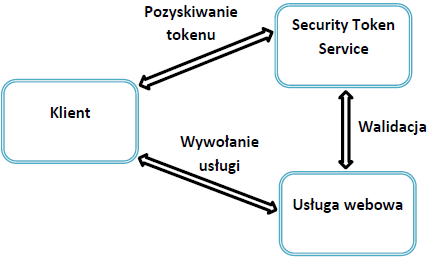
\includegraphics{img/ws-trust.png}
			\caption{Model zapewnienia bezpieczeństwa dostępu do aplikacji w standardzie WS-Trust}
			\label{Model zapewnienia bezpieczeństwa dostępu do aplikacji w standardzie WS-Trust}
		\end{figure}

		Klient może pozyskiwać tokeny bezpieczeństwa od usługi ,,Security Token Service''. Otrzymany token może być dołączony do żądania klienta wysyłanego do usługi webowej. Serwis powinien weryfikować czy usługa wystawiająca token objęta jest relacją zaufania względem danych, które dostarcza. Serwis może ufać otrzymywanym tokenom bezpieczeństwa lub zlecać ich walidację usłudze STS. Usługa może również komunikować się z modułem STS w celu wymiany otrzymanego tokenu bezpieczeństwa na inny odpowiedni dla mechanizmów bezpieczeństwa danej usługi. 

		Serwis może deklarować kryteria dla otrzymywanych tokenów określające kiedy token będzie uznany za zaufany\cite{WS-Trust-1.4-with-errata}. Możliwe kryteria to np.:

		\begin{itemize}
			\item typ tokenu(np. token protokołu Kerberos)
			\item dostawca tokenu - usługa deklaruje dostawców tokenów, dla których istnieje relacja zaufania
			\item hierarchia zaufania - usługa może określać zaufanie względem jednostek, w których hierarchii zaufania znajduje się określony serwis
			\item zaufanie tylko dla tokenów wystawianych przez serwis uwierzytelniający - otrzymane tokeny przekazywane są do usługi uwierzytelniającej; w procesie udostępniania zasobów wykorzystywany jest token wygenerowany przez tą usługę na podstawie tokenu dostarczonego w żądaniu. 
		\end{itemize} 
		
	Informowanie odbiorców usług o wymaganiach bezpieczeństwa stawianych przez serwis jest możliwe dzięki standardowi WS-SecurityPolicy. Jest to specyfikacja rozszerzająca język WSDL(Web Services Description Language) pozwalająca definiować następujące wymagania bezpieczeństwa:

	\begin{itemize}
		\item konieczność dostarczenia tokenu bezpieczeństwa
		\item konieczność dostarczenia podpisu dla tokenu bezpieczeństwa
		\item wymagany sposób szyfrowania
		\item konieczność dostarczenia cyfrowego podpisu dla określonej części wiadomości
		\item konieczność szyfrowania określonej części wiadomości
		\item wymaganie dostarczenia określonych wiadomości opisujących klienta aplikacji
	\end{itemize} 

	\subsection{Standard WS-Federation}

		Standard WS-Federation definiuje mechanizmy pozwalające na dzielenie tożsamości i atrybutów jednostek pomiędzy usługami w różnych domenach administracyjnych lub domenach bezpieczeństwa w oparciu o reguły i wymagania zdefiniowane przy pomocy mechanizmu polityk\cite{Goodner09}. Specyfikacja określa sposób współdzielenia informacji dotyczących bezpieczeństwa pomiędzy usługami dostarczającymi tokenów bezpieczeństwa a dostawcami usług. Definicja polityk umożliwia deklarację danych, które mogą być współdzielone. Wymieniane informacje mogą obejmować dane o sfederowanych usługach, wymagania zawarte w politykach federacji, opis relacji zaufania oraz tokeny bezpieczeństwa.

		Koncepcja federacji w standardzie WS-Federation wprowadza mechanizm mapowania tożsamości. Jest to proces translacji cyfrowej tożsamości pomiędzy formatem rozumianym przez domenę nadawcy a formatem akceptowanym przez domenę docelową. Usługa dokonująca mapowania tożsamości powinna posiadać relację zaufania dla domeny nadawcy i mieć uprawnienia do przekazywania informacji do domeny odbiorcy.

		Specyfikacja WS-Federation wykorzystuje model pozyskiwania tokenów bezpieczeństwa i uwierzytelniania przy ich pomocy opisywany w standardzie WS-Trust. Standard WS-Federation rozszerza koncepcję opisaną w WS-Trust o możliwość pozyskiwania informacji o politykach realizowanych przez usługi i stawianych przez nie wymaganiach dotyczących zabezpieczania dostępu do chronionych zasobów. Specyfikacja określa sposób wykorzystania modeli opisanych przez WS-Security, WS-Trust i WS-Policy tworząc bardziej rozbudowany model relacji zaufania pomiędzy serwisami przy użyciu mechanizmu federacji.

		\begin{figure}[h]
			\centering
				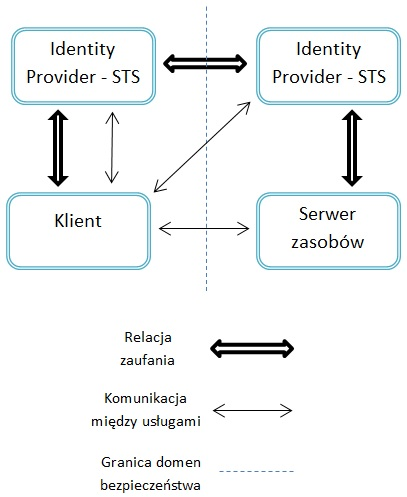
\includegraphics{img/ws-federation.jpg}
			\caption{Prosty scenariusz federacji serwisow}
			\label{Prosty scenariusz federacji serwisów}
		\end{figure}

		Przedstawiony schemat ilustruje przebieg uzyskiwania dostępu do zasobu przy użyciu mechanizmu federacji. Przerywana linia stanowi granicę między domenami bezpieczeństwa. Klient przeprowadza proces uwierzytelniania  i uzyskuje token bezpieczeństwa od usługi ,,Security Token Service'' w swojej domenie bezpieczeństwa. Otrzymany token zostaje przedstawiony usłudze STS w odrębnej domenie bezpieczeństwa w celu uzyskania tokenu uprawniającego do dostępu do zasobów w tej domenie. Token uzyskany w tym procesie jest przesyłany w żądaniach dostępu do zasobów w odrębnej domenie bezpieczeństwa. 

	\subsection{Standard OAuth}

		W podstawowej koncepcji ograniczania dostępu do zasobów użytkownik uzyskuje dostęp do zasobów korzystając z dany uwierzytelniających właściciela zasobu. Gdy klient usługi chce udostępnić usłudze chronione zasoby musi przekazać jej swoje dane uwierzytelniające.  Zastosowanie tego modelu pociąga za sobą zagrożenia bezpieczeństwa związane z przechowywaniem danych uwierzytelniających przez usługę, której udzielono dostępu do danych, brakiem możliwości ograniczenia udzielonych praw dostępu jedynie do części zasobów oraz brakiem możliwości odebrania przydzielonych wcześniej praw dostępu.

		Jednym z rozwiązań tego typu problemów jest zastosowanie standardu OAuth - specyfikacji definiującej mechanizmy autoryzacji dostępu do zasobów dla protokołu HTTP\cite{Hardt12}. Standard OAuth zakłada wprowadzenie dodatkowej warstwy autoryzacji  oraz rozdzielenie ról klienta i właściciela zasobu. W procesie przyznawania klientowi praw dostępu do zasobu wykorzystywane są dane uwierzytelniające różne od danych właściciela zasobu. W tym celu klient otrzymuje token dostępu od serwera autoryzującego za zgodą właściciela zasobu. Token zawiera m. in. informacje określające zakres praw nadanych użytkownikowi oraz okres obowiązywania przyznanych uprawnień. 

		Właścicielem zasobów w standardzie OAuth jest jednostka przyznająca dostęp do zasobów. Klientem jest aplikacja, która w odpowiedzi na operacje wykonywane przez  właściciela zasobu i za jego zgodą korzysta z tego zasobu.

		\begin{figure}[h]
			\centering
				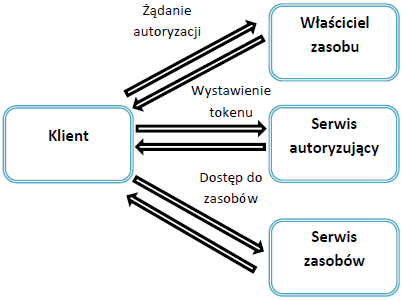
\includegraphics{img/oauth.png}
			\caption{Przebieg autoryzacji w standardzie OAuth}
			\label{Przebieg autoryzacji w standardzie OAuth}
		\end{figure}

		Proces przyznania klientowi dostępu do zasobu rozpoczyna się żądaniem autoryzacji przesyłanym do właściciela zasobu.  Właściciel zasobu odpowiada na żądanie przesyłając grant autoryzujący typu zależnego od metody wykorzystywanej do autoryzacji. Następnie klient przysyła do serwera autoryzującego żądanie przydzielenia tokenu dostępu na podstawie otrzymanego grantu autoryzującego. Serwer autoryzujący uwierzytelnia klienta i weryfikuje otrzymany grant autoryzujący i na tej podstawie przyznaje token dostępu. Klient korzysta z zasobów przedstawiając przydzielony mu token dostępu.

%---------------------------------------------------------------------------

\autsection{Mechanizmy zapewniania poufności i integralności komunikacji}{Tomasz Wójcik}
\label{sec:poufnosc}
\subsection{Transport Layer Security}

Protokół Transport Layer Security służy do zapewnienia poufności i integralności danych przesyłanych przez sieć publiczną. Pozwala także na potwierdzenie tożsamości serwera i opcjonalnie klienta, na podstawie certyfikatów X.509. Transport Layer Security może zabezpieczać protokoły warstwy aplikacji modelu TCP/IP takie jak HTTP, FTP, LDAP czy IMAP. 
TLS wywodzi się z protokołu Secure Sockets Layer, stworzonego w 1994 roku w firmie Netscape do zabezpieczania transakcji w systemie WWW. Trzecia wersja tego protokołu posłużyła do stworzenia przez IETF standardu Transport Layer Security. 

TLS może być podzielony na dwie warstwy: warstwę handshake i warstwę record\cite{citeulike:6536152}. Warstwa handshake składa się z trzech podprotokołów. Protokół handshake służy do wymiany informacji niezbędnych do nawiązania bezpiecznego połączenia oraz negocjacji parametrów sesji pomiędzy klientem a serwerem. Protokół change cipher spec służy do powiadamiania odbiorcy o zmianie klucza. Protokół alert ma na celu powiadamianie o zmianie statusu połączenia lub błędach. 

Warstwa record obsługuje podprotokół o tej samej nazwie. Służy on do właściwego zabezpieczania danych które mają zostać wysłane przez sieć. Otrzymuje on wiadomości z warstwy aplikacji, dzieli je na bloki, opcjonalnie kompresuje dane, oblicza MAC(Message Authentication Code), szyfruje i przekazuje do warstwy transportowej. Z kolei otrzymane dane są deszyfrowane, weryfikowane, dekompresowane, łączone w całość i dostarczane do klienta warstwy wyższej. 

\subsubsection{Przebieg typowej negocjacji parametrów sesji przy użyciu protokołu handshake}

		\begin{figure}[!htb]
			\centering
				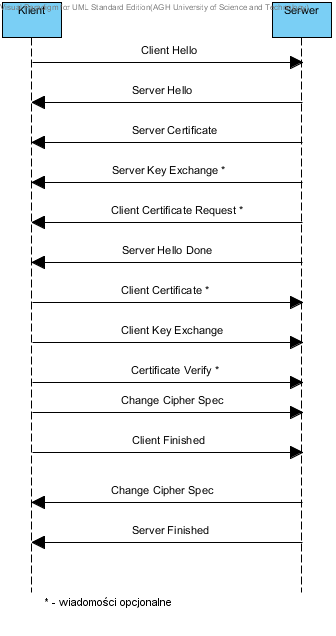
\includegraphics{img/HandshakeTLS.png}
			\caption{Wiadomości wymieniane między klientem i serwerem podczas procedury handshake w protokole Transport Layer Security}
			\label{Wiadomości wymieniane między klientem i serwerem podczas procedury handshake w protokole Transport Layer Security}
		\end{figure}

Klient rozpoczyna fazę handshake wysyłając wiadomość typu Client Hello\cite{MSTLS03}. Zawiera ona numer wersji protokołu, pewne losowe dane, które służą do stworzenia klucza sesyjnego oraz zbiór obsługiwanych przez klienta algorytmów służących do wymiany kluczy, do szyfrowania, do obliczania funkcji skrótu oraz opcjonalnie do kompresji. Ponieważ tworzenie nowej sesji jest kosztowną operacją, klient może wysłać identyfikator poprzedniej sesji w celu jej wznowienia.

Serwer odpowiada wiadomością Server Hello. Zawiera ona informację o najwyższej wersji protokołu oraz najsilniejszym zestawie algorytmów wspieranych zarówno przez serwer jak i klienta. Serwer zwraca także identyfikator sesji, który może posłużyć do jej późniejszego wznowienia oraz losowe dane.
Serwer wysyła kolejną wiadomość Server Certificate, zawierającą certyfikat serwera. Klient na podstawie certyfikatu wydanego przez zaufany CA może potwierdzić tożsamość serwera, może także sprawdzić zgodność domeny certyfikatu oraz domeny z którą się łączy. Typowo certyfikat zawiera także klucz publiczny który służy do zaszyfrowania tzw. premaster secret. Jeżeli certyfikat nie zawiera klucza publicznego, serwer tworzy tymczasową parę kluczy i wysyła klucz publiczny w osobnej wiadomości Server Key Exchange. Jeżeli serwer wymaga także uwierzytelnienia klienta na podstawie jego certyfikatu, wysyła kolejną wiadomość, typu Client Certificate Request. Wiadomość Server Hello Done wskazuje na to, że serwer zakończył tę fazę i czeka na odpowiedź klienta.

Jeżeli jest to wymagane, klient wysyła serwerowi swój certyfikat przy użyciu wiadomości typu Client Certificate. Następnie, w każdym przypadku wysyła wiadomość Client Key Exchange, zawierającą tzw. premaster secret wygenerowany z obu wartości losowych przesłanych w fazie Hello. Sekret ten jest szyfrowany kluczem publicznym serwera. Wiadomość ta zawiera też ponownie numer wersji protokołu. Jest to zabezpieczenie przed atakiem typu rollback, czyli podmianie wersji na mniej bezpieczną w początkowej wiadomości Client Hello. Wiadomość Certificate Verify jest wysyłana tylko gdy wymagane jest uwierzytelnienie klienta. Klient podpisuje kluczem publicznym skrót wszystkich wiadomości wymienionych do tej pory podczas fazy handshake i wysyła go do serwera. Wiadomość Change Cipher Spec z podprotokołu o tej samej nazwie jest następnie wysyłana w celu powiadomienia o zmianie klucza szyfrowania. Wiadomość Client Finished zawiera skrót całej konwersacji, jest to pierwsza wiadomość szyfrowana kluczem sesyjnym, przechodząca przez warstwę Record. 

Serwer również używa wiadomości Change Cipher Spec, potwierdzając zmianę klucza. Procedurę handshake kończy wiadomość Server Finished. Analogicznie do podobnej wiadomości wysyłanej przez klienta, zawiera ona wartość skrótu dla wszystkich wiadomości wymienionych dotychczas pomiędzy klientem i serwerem.


\subsection{XML Encryption}

Protokół Transport Layer Security może zapewnić bezpieczeństwo komunikacji pomiędzy dwoma węzłami w sieci publicznej. Jednak w niektórych przypadkach nie jest to wystarczające. W systemach typu SOA serwisy mogą być ze sobą w różny sposób łączone. Utworzona w ten sposób pojedyncza usługa wyższego rzędu może grupować wiele serwisów, potencjalnie znajdujących się w różnych domenach bezpieczeństwa, np. w celu dostarczenia użytkownikowi wygodnego interfejsu obsługującego cały proces biznesowy. Co za tym idzie, nie wszystkie dane wysyłane do danej usługi są przeznaczone bezpośrednio dla niej. Jeżeli klient chce zabezpieczyć część swoich danych przed ich odczytaniem lub podmianą przez serwis który pośredniczy w dostarczeniu ich do docelowej usługi, musi skorzystać z mechanizmów bezpieczeństwa działających na poziomie wiadomości, a nie kanału transmisji danych.

Jednym ze standardów tego typu jest XML Encryption. Opisuje on reguły szyfrowania wiadomości w języku XML. Standard ten umożliwia szyfrowanie wybranych fragmentów wiadomości, zachowuje składnię języka XML, pozwalając na przetwarzanie wiadomości przez węzły nie obsługujące standardu oraz pozwala na dodanie metadanych opisujących jakie mechanizmy szyfrowania zostały, grupując w wiadomości wszystkie elementy potrzebne do jej odszyfrowania.\cite{kanneganti2008soa}
Tym samym XML Encryption pozwala na zagwarantowanie poufności danych przetwarzanych przez złożone usługi w modelu SOA.

\lstset{language=XML, caption={Struktura przykładowego elementu zaszyfrowanego przy użyciu XML Encryption}, captionpos=b, label=XMLEncryption}
		\begin{lstlisting}
<EncryptedKey xmlns="http://www.w3.org/2001/04/xmlenc#">
	<EncryptionMethod 
	Algorithm="http://www.w3.org/2001/04/xmlenc#rsa-1_5"/>
	<ds:KeyInfo xmlns:ds="http://www.w3.org/2000/09/xmldsig#">
		<ds:KeyName>Nazwa klucza</ds:KeyName>
	</ds:KeyInfo>
	<CipherData>
		<CipherValue>S0xVQ1pQVUJMSUNaTlk=</CipherValue>
	</CipherData>
	<ReferenceList>
		<DataReference URI="#ZaszyfrowaneDane1"/>
	</ReferenceList>
</EncryptedKey>
		
		
<EncryptedData xmlns="http://www.w3.org/2001/04/xmlenc#"
	Type="http://www.w3.org/2001/04/xmlenc#Element"
	Id="ZaszyfrowaneDane1"/>
	<EncryptionMethod 
	Algorithm="http://www.w3.org/2001/04/xmlenc#tripledes-cbc"/>
	<ds:KeyInfo xmlns:ds="http://www.w3.org/2000/09/xmldsig#">
		<ds:KeyName>Nazwa klucza</ds:KeyName>
	</ds:KeyInfo>
	<CipherData>
		<CipherValue>VEFKTkVEQU5F</CipherValue>
	</CipherData>
</EncryptedData>
\end{lstlisting}

XML Encryption pozwala na zastosowanie szyfrowania symetrycznego, asymetrycznego lub hybrydowego. 
Zaszyfrowane dane są zamieniane na element XML o nazwie \texttt{EncryptedData}. Atrybut \texttt{Type} tego elementu wskazuje na typ zaszyfrowanych danych. Standard umożliwia szyfrowanie całego elementu XML lub jego zawartości. Element ten zawiera też swój unikalny identyfikator, który pozwala na odnoszenie się do niego z innych elementów zawierających metadane na temat szyfrowania. \texttt{EncryptedData} zawiera element \texttt{EncryptionMethod} który informuje o algorytmie szyfrującym. Dostępne są zarówno algorytmy symetryczne(np. AES) jak i asymetryczne(np. RSA). Element \texttt{CipherData} przechowuje zaszyfrowane dane, zakodowane przy użyciu Base64 wewnątrz elementu \texttt{CipherValue}. Możliwe jest też odniesienie się do danych znajdujących się w zewnętrznej lokalizacji przy pomocy elementu \texttt{CipherReference}.
Jeżeli klucz służący do szyfrowania danych nie jest został uprzednio ustalony, konieczne jest zastosowanie elementu \texttt{EncryptedKey}. Element ten może zostać umieszczony wewnątrz elementu \texttt{EncryptedData} lub w dowolnym innym miejscu w dokumencie, w przypadku wiadomości SOAP najczęściej w nagłówku WS-Security.
W najbardziej typowym przypadku wykorzystania szyfrowania hybrydowego, \texttt{EncryptedKey} zawiera wygenerowany przez nadawcę klucz sesji zaszyfrowany przy pomocy klucza publicznego odbiorcy. Element \texttt{EncryptionMethod} wskazuje na algorytm, którym został zaszyfrowany klucz sesyjny, zaś element \texttt{KeyInfo} służy do identyfikacji klucza publicznego użytego w tym algorytmie. Możliwe jest przesłanie wykorzystanego certyfikatu(wewnątrz tego elementu lub w załączniku SOAP) lub wskazanie na konkretny klucz przy użyciu jego identyfikatora lub Distinguished Name certyfikatu zawierającego ten klucz. Wynik działania algorytmu szyfrującego jest umieszczony w elemencie \texttt{CipherData}, zawiera on zaszyfrowany asymetrycznie klucz sesyjny. 
Ponieważ wiadomość może zawierać części przeznaczone do odszyfrowania przez różnych nadawców istotne jest wskazanie które elementy \texttt{EncryptedData} powinny zostać odszyfrowane przez danego nadawcę. Element \texttt{ReferenceList} zawiera listę elementów \texttt{DataReference} zawierających numery identyfikacyjne elementów \texttt{EncryptedData}. 
Każdemu z odbiorców zaszyfrowanej części wiadomości odpowiada jeden element \texttt{EncryptedKey}. Odbiorca jest identyfikowany na podstawie danych z elementu \texttt{KeyInfo} lub opcjonalnego atrybutu \texttt{Recipient}, który jednak nie ma standardowej postaci. \cite{Eastlake:02:XES} 
Standard umożliwia jednokrotne szyfrowanie wiadomości przeznaczonej dla wielu odbiorców, jednak klucz szyfrujący musi zostać zaszyfrowany wielokrotnie przy pomocy kluczy publicznych wszystkich odbiorców lub ustalony wcześniej. 


\subsection{XML Signature}

Standard XML Encryption gwarantuje poufność danych na poziomie wiadomości. Dzięki temu węzły pośredniczące w transmisji wiadomości do odbiorcy końcowego nie mogą odczytać jej zaszyfrowanych fragmentów. Wciąż jednak mogą one dowolnie modyfikować wiadomość, w tym także zmieniać jej zaszyfrowane części. Integralność wiadomości może być zapewniana w różny sposób. W protokole Transport Layer Security jest ona realizowana przy użyciu kodów uwierzytelniania wiadomości (ang. Message authentication code). Algorytmy MAC na podstawie wiadomości i wspólnego dla nadawcy i odbiorcy klucza tworzą kod, który jest dołączany do wiadomości przez nadawcę i może następnie w celu weryfikacji zostać odtworzony przez odbiorcę. Inną możliwością zapewnienia integralności wiadomości jest wykorzystanie podpisów cyfrowych: nadawca podpisuje wiadomość swoim kluczem prywatnym, natomiast odbiorca może zweryfikować integralność wiadomości przy pomocy klucza publicznego nadawcy. Podpis cyfrowy wiadomości, dzięki wykorzystaniu klucza prywatnego znanego wyłącznie nadawcy, zapewnia także jej niezaprzeczalność (ang. non-repudation). Oznacza to, że nadawca nie może zaprzeczyć faktu nadania określonej wiadomości, co może mieć znaczenie podczas rozstrzygania sporów prawnych. MAC nie gwarantuje niezaprzeczalności wiadomości, ponieważ wykorzystywany klucz jest znany obu komunikującym się stronom.

Standard XML Signature wykorzystuje podpis cyfrowy do zagwarantowania integralności i niezaprzeczalności wiadomości. Podobnie jak XML Encryption jest zorientowany na wiadomości w formacie XML i analogicznie umożliwia podpisywanie wybranych fragmentów wiadomości oraz definiuje sposób przekazywania metadanych opisujących mechanizmy zastosowane w celu uzyskania podpisu.

Dodatkowym problemem, który nie występuje przy szyfrowaniu dokumentów w języku XML jest związany możliwością przetwarzania podpisanych fragmentów wiadomości przez wiele węzłów. Język XML pozwala na zapisanie tej samej semantycznie wiadomości na wiele różnych sposobów, różniących się np. kodowaniem, formatowaniem, kolejnością atrybutów czy definicjami przestrzeni nazw. Jeżeli węzeł pośredni ma za zadanie przeniesienie podpisanego fragmentu do innej wiadomości, z dużym prawdopodobieństwem operacja taka zmieni sekwencję bajtów związaną z podpisywanym fragmentem. Ponieważ algorytmy służące do podpisów cyfrowych podpisują określoną sekwencję bajtów, weryfikacja fragmentu wiadomości u jego końcowego odbiorcy zakończyłaby się niepowodzeniem. Problem ten można rozwiązać sprowadzając podpisywany fragment dokumentu XML do postaci kanonicznej. 

Operacja ta jest zdefiniowana w standardzie XML canonicalization. Przyjmuje ona poprawny składniowo (ang. well-formed) dokument XML lub jego fragment i tworzy równoważny dokument standardowy\cite{Boyer:01:CXV}. Sprowadzanie do postaci kanonicznej opiera się o poniższy zestaw reguł, które można wykonywać w dowolnej kolejności:
\begin{itemize}
\item Zamiana kodowania na UTF-8
\item Ujednolicenie nowych linii jako \#xA (line feed)
\item Usunięcie opcjonalnych deklaracji XML i DTD
\item Zamiana referencji znaków niebędących znakami specjalnymi na odpowiadające im znaki
\item Usunięcie CDATA i zastąpienie znaków specjalnych ich referencjami
\item Zamiana pustych znaczników elementów na pary znaczników (np. zamiana <a/> na <a></a>)
\item Usunięcie białych znaków wewnątrz znaczników oraz na początku i końcu dokumentu
\item Zamiana apostrofów na cudzysłowy
\item Ujednolicenie wartości atrybutów: zamiana referencji i usuniecie nadmiarowych białych znaków
\item Dodanie znanych atrybutów domyślnych
\item Uszeregowanie atrybutów zgodnie z URI ich przestrzeni nazw i nazwą lokalną
\item Usunięcie nadmiarowych definicji przestrzeni nazw, sortowanie tak samo jak w przypadku atrybutów
\end{itemize}

\lstset{language=XML, caption={Przykład zastosowania XML Inclusive Canonicalization}, captionpos=b, label=InclusiveCanonicalization}
		\begin{lstlisting}
<quote xmlns:ns1="http://manning.com/xmlns/samples/soasecimpl" 
xmlns:soapenv="http://schemas.xmlsoap.org/soap/envelope/" 
xmlns:xsd="http://www.w3.org/2001/XMLSchema" 
xmlns:xsi="http://www.w3.org/2001/XMLSchema-instance" 
xsi:type="xsd:float">103.25</quote>
		\end{lstlisting}
		
\lstset{language=XML, caption={Przykład zastosowania XML Exclusive Canonicalization}, captionpos=b, label=ExclusiveCanonicalization}
		\begin{lstlisting}
<quote xmlns:xsi="http://www.w3.org/2001/XMLSchema-instance" 
xsi:type="xsd:float">103.25</quote>
		\end{lstlisting}

Najbardziej  problematyczną częścią sprowadzania XML do postaci kanonicznej jest obsługa przestrzeni nazw. Twórcy standardu XML canonicalization zadecydowali, że dokumenty różniące się wyłącznie prefiksami elementów, mimo, że prefiksy w obu dokumentach odnoszą się do przestrzeni nazw z tym samym URI, będą traktowane jak różne dokumenty. Poważniejszy problem pojawia się w sytuacji, gdy jedynie fragment wiadomości ma zostać sprowadzony do postaci kanonicznej, co występuje często podczas użycia XML Signature. Pierwotny standard przewidywał dopisanie do głównego elementu danego fragmentu wszystkich przestrzeni nazw zdefiniowanych w elementach nadrzędnych, także tych nieużywanych przez dany fragment wiadomości. W przypadku gdy taki fragment zostanie umieszczony w innej wiadomości, wewnątrz elementu korzystającego z innych przestrzeni nazw, postać kanoniczna tego fragmentu zmieni się, mimo tego, że zawartość fragmentu nie uległa zmianie. Problem ten wymusił stworzenie standardu Exclusive XML Canonicalization, który uwzględnia w wyniku tylko te przestrzenie nazw, które są używane w prefiksach elementów i atrybutów fragmentu wiadomości na którym przeprowadzana jest ta operacja\cite{Boyer:02:EXC}. Przestrzenie nazw mogą być także używane w sposób niebezpośredni w wartościach elementów, co może stanowić lukę bezpieczeństwa. Dlatego przestrzenie takie powinny zostać uwzględnione w dodatkowym parametrze InclusiveNamespaces, który wymusza ich dodanie do postaci kanonicznej.
	
Dane związane z podpisem cyfrowym są przechowywane w elemencie \texttt{Signature}\cite{Eastlake:08:XSS}, który w przypadku wiadomości SOAP jest najczęściej umiejscowiony w nagłówku SOAP definiowanym przez WS-Security. Z uwagi na ilość metadanych opisujących co i w jaki sposób jest podpisywane, struktura tego elementu jest złożona. Element \texttt{SignatureInfo} zawiera listę elementów \texttt{Reference}, które odpowiadają poszczególnym podpisywanym fragmentom wiadomości. Każdy taki element posiada odnośnik do podpisanego elementu i określa sposób sprowadzenia do postaci kanonicznej, a także zastosowaną funkcję skrótu i wartość skrótu elementu zapisaną przy użyciu Base64, gdyż względy wydajnościowe związane z kryptografią asymetryczną powodują, że najczęściej fragmenty XML nie są bezpośrednio podpisywane. Elementem na którym w rzeczywistości jest przeprowadzana operacja podpisywania jest \texttt{SignedInfo}. W związku z tym, musi on również zdefiniować swoją formę kanoniczną oraz zastosowaną funkcję skrótu. Obliczona wartość podpisu tego elementu, również zakodowana w Base64,  jest umieszczana wewnątrz znacznika \texttt{SignatureValue}. Element \texttt{KeyInfo} zawiera klucz publiczny podpisującego lub referencję do niego, stanowiąc ostatni wymagany element do zweryfikowania podpisu po stronie nadawcy.
